\documentclass[12pt, class=report, crop=false]{standalone}
\usepackage{ba_thesis}

\begin{document}

\chapter{Plasma Physics}%
\label{chap:plasma}

\section{The Definition of Plasma}
It is common that people, when asked about what is plasma, their definition stops at the fact that it is a \textbf{partially ionized gas}. But this is just one of the three defining characteristics. After all, even the air is partially ionized. The other two proprties that a medium should satisfy in order to be considered plasma are quasi-neutrality and collective behaviour.

To be \textbf{quasi-neutral} means that the medium has an equal number of positive and negative charges in its entire volume, but small deviations from neutrality are possible locally. That is, if \(n_p\), \(n_e\) are the positive charge density and the electron density, respectively, in the whole region of the plasma we have \(n_p = n_e\), yet in small regions in the space inside we have \(n_p \approx n_e\). A small remark should be made here. While I say that the plasma as a whole is neutral, it is so by approximation still. If one starts building plasma by pumping energy into a gaseous medium for example, some of the first ionized electrons can actually escape the medium. It is only after a certain positive charge density has been achieved that no electrons can not escape anymore due to Coulomb attraction. Once enough ionization electrons are produced, the charge imbalance becomes incredibly small (\textit{i}.\textit{e}. \(\frac{n_p - n_e}{n_e}\ll 1\)). This is though a very hard to observe charge imbalance in practice, so we can say that plasma as a whole is neutral. The localized imbalance in turn is not constantly small; it can vary widely due to the disordered motion of the constituent particles, but statistically speaking neutrality is maintained locally when we look at the time averages.

\textbf{Collective behaviour} is a consequence of the fact that the main type of interaction between the particles constituting the plasma, namely Coulomb interaction, is long range. As such, we can say that any particle in the plasma feels all the other ones. This leads to many important properties specific to plasma, like particle and momentum transport. The simplest response is plasma oscillation, which arises when plasma is placed in a constant electric field. The electrons are pushed by the electric field, but the surplus of positive charge left behind pulls them back, creating an oscillatory motion (we should take into consideration that the positive ions are at least a couple thousand times heavier than the electrons, so it is harder to influence their motion).This property also influences the the way in which plasma interacts with electromagnetic radiation, giving rise to radiation transport phenomena for example.

It is important to note from the very begining that in a plasma we have quite many different species of particles. The most simple model would only include electrons, neutral atoms and ions that have just one missing electron, but in reality we can have all the possible types of ions (so also with two or more missing electrons) and photons (which arise from the excitations and de-excitations that happen in this very energetic medium).

In the following sections we aim to go deeper into the parameters that characterize plasmas and the basic models for it. The discussion brings together ideas from~\cite{karschApplicationsHighIntensity2018} and~\cite{mulserHighPowerLasermatter2010}.

\section{Temperature}
We would like now to study the statistics of electrons. First of all, we should realize that the interparticle distances in plasmas are quite large, but also the temperature needed to sustain ionization is quite high. So high in fact that working with the Fermi-Dirac statistics is not necesary, since this quantum mechanically derived distribution can be approximized very well by the classical Maxwell-Boltzmann distribution in this particular situation.

The number of electron with x-axis velocity between \(v_{e,x}\) and \(v_{e,x}+\dd{v_{e,x}}\) is then given by

\begin{equation}
  f_e (v_{e,x}) \dd{v_{e,x}} = n_e \sqrt{\frac{m_e}{2\pi K_B T_e}} \ee^{-\frac{K_x}{K_B T_e}}\,,
\end{equation}
where \(n_e\), \(m_e\) and \(T_e\) are the electrons' density, mass and temperature, respectively, \(K_B\) is the Boltzmann constant and \(K_x = \frac{m_e v_{e,x}^2}{2}\) is the kinetic energy of the photons. The normalization constant was obtained from the electron density, since \(n_e = \int_{-\infty}^{+\infty} \dd{v_{e,x}} f_e (v_{e,x})\). This gives an average kinetic energy of

\begin{equation}
  K_x^{avg} = \frac{\int_{-\infty}^{+\infty} \dd{v_{e,x}} K_x f_e (v_{e,x})}{\int_{-\infty}^{+\infty} \dd{v_{e,x}} f_e (v_{e,x})} = \frac{m_e}{2 n_e} \int_{-\infty}^{+\infty} \dd{v_{e,x}} v_{e,x}^2 f_e (v_{e,x}) = \frac{1}{2} K_B T_e\,.
\end{equation}

This is extended in 3D easily, since the distribution of velocity in this case should not have any preferential direction

\begin{equation}
  K^{avg} = \frac{3}{2} K_B T_e\,.
\end{equation}
As it can be seen, we can basically treat the electrons inside the plasma as we would an ideal gas and we have obtained that the average kinetic energy is proportional to the temperature.

A simple numerical application shows us that in order to have \(K_B T_e = 1\) eV, the temperature would be around \(11600\) K. Thus, since the ionized electrons are above the energy level of outer bounded states (so above 1 eV), using Kelvin or degrees Celsius is not that handy. In practice, we will rather use eV (energy units) temperature, which is to be converted to the usual temperature by dividing to \(K_B\).

We could actually treat the ions and the neutral atoms inside the plasma in the same manner. Considering this, we must make the remark that we can have different temperature scales in plasmas. While at thermodynamic equilibrium the system of electrons, ions and neutrals should have a uniform temperature, under the action of an electric field, lets say, the motion of the electrons is influenced more than that of the ions due to the difference in mass, while the neutrals are not affected at all, so we have \(T_n\neq T_i\neq T_e\). Of course, equilibration between species can be achieved through collisions or radiation emission and absorption. In complete models, one should also consider the temperatures of photons and individual ion subspecies that can appear. Considering this, in general, thermal equilibration can take a long time. It is also important to visualize that the temperature can be directionally dependent depending on the orientation of the fields we apply.

\section{Debye Shielding}
In this section we will derive a common criterion for quasi-neutrality. Let us consider an infinite medium filled with plasma at thermal equilibrium, \(T=T_e = T_i\) and with one ion species with charge \(Ze\), such that we have \(n_e = Zn_i\). We are interested to see what happens if we introduce an infinite plane with constant positive surface charge density \(\sigma\) in this system (see~\cref{fig:debye}).

\begin{figure}[h]
  \centering
  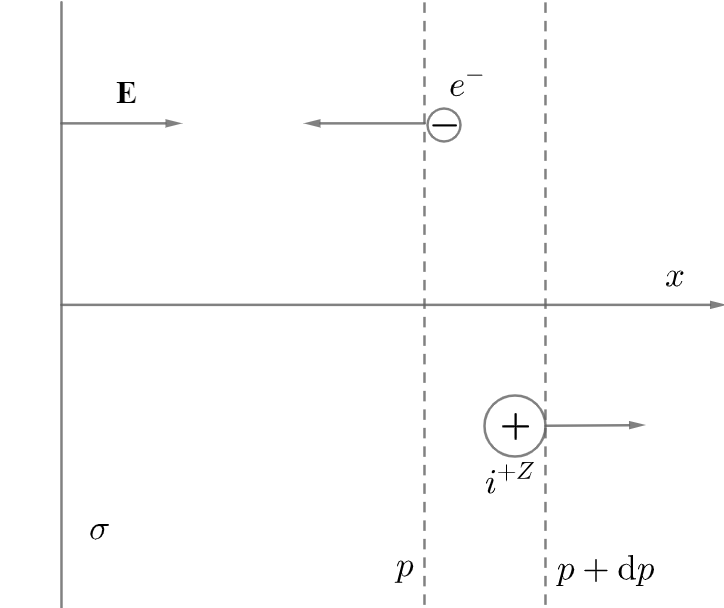
\includegraphics[width=0.52\textwidth]{Debye}%
  \caption{A schematic figure that shows the action of introducing the charged sheet in the plasma}\label{fig:debye}%
\end{figure}

The constant electric \(E = \frac{\sigma}{2\varepsilon_0}\) generated by the plate will act to locally separate sheets of electrons and ions, until equilibrium between the pressures \(p_e = n_e K_B T\) and \(p_i = n_i K_B T \) is achieved. For the electrons in a sheet of thickness \(\delta x\) we have

\begin{equation}
  \dd{p_e} = K_B T \dd{n_e} = -e n_e E \delta x\,,
\end{equation}
which can be rewritten as

\begin{equation}
  \frac{1}{n_e} \partial_x n_e = - \frac{e}{K_B T} E = \frac{e}{K_B T} \partial_x \phi\,,
\end{equation}
where \(\phi\) is the electrostatic potential. Solving this equation for the density of electrons, we obtain

\begin{equation}
  n_e(x) = \bar{n}_e \ee^{\frac{e\phi}{K_B T}},\; \bar{n}_e = n_e(x \rightarrow \infty)\,.
\end{equation}
In the same manner one obtains a similar expression for the ion density

\begin{equation}
  n_i (x) = \frac{\bar{n}_e}{Z} \ee^{-\frac{Ze\phi}{K_B T}}\,.
\end{equation}

Writing the Poisson equation in terms of these results gives us

\begin{equation}
  \partial_x^2 \phi = \frac{e \bar{n}_e}{\varepsilon_0} \left(\ee^{\frac{e\phi}{K_B T}} - \ee^{-\frac{Ze\phi}{K_B T}} \right)\,.
\end{equation}
If the potential energy arising from the field is small compared the the kinetic energy of the particles in the plasma, \textit{i}.\textit{e}. \(e\phi\ll K_B T\), the potential equation can be simplified in approximation to

\begin{equation}
  \partial_x^2 \phi = \frac{e \bar{n}_e}{\varepsilon_0} \left( 1 +\frac{e\phi}{K_B T} -1 + \frac{Ze\phi}{K_B T}\right) = \frac{e^2 \bar{n}_e (Z+1)}{\varepsilon_0 K_B T} \phi\,.
\end{equation}
Obtaining the solution if this is trivial

\begin{equation}
  \phi(x) = \phi_0 \ee^{-\frac{x}{\lambda_D}}\,,
\end{equation}
where we introduced the Debye length

\begin{equation}
  \lambda_D = \sqrt{\frac{\varepsilon_0 K_B T}{\bar{n}_e e^2 (Z+1)}}\,.
\end{equation}
This shows us that at a distance of \(\lambda_D\) away from the plate, the electric field generated by it, as well as the corresponding potential, is screened by about 63\%. This offers us great insight in how to obtain quasi-neutrality.

From this discussion we can conclude that quasi-neutrality holds if the spatial extension of our ionized gas is at least a couple times larger than the Debye length, since in this case the local deviations from neutrality \(n_p\approx n_e\) are screened. For dimensions smaller than \(\lambda_D\), there is no quasi-neutrality very high-intensity localized fields can occur giving rise to interesting physical phenomena.

In practice, one uses another form for \(\lambda_D\) which neglects the \(Z\) and uses the temperature and particle density with more convenient units

\begin{equation}
  \lambda_D = \sqrt{\frac{\varepsilon_0 K_B T}{\bar{n}_e e^2}} = 6.9 \sqrt{\frac{T_e [\textrm{K}]}{n_e [\textrm{cm}^3 ]}}\,,
\end{equation}
the last expression giving \(\lambda_D\) in cm.

\section{Plasma Frequency}


\section{Electromagnetic Waves in Plasma}
\section{The Vlasov Equation}
\section{Two Stream Instability}
\end{document}
